%!TEX root = ../dissertation.tex

\chapter{Evaluation}
\label{chapter:evaluation}
% Introduce evaluation...
% Main goals
% Setup used
The evaluation focused on two aspects.
First, we need to verify if the method to get the distance from a given beacon is reliable.
Second, since we have a service running in background scanning for beacons from time to time we evaluated our solution in terms of battery consumption.

In section \ref{sec:evaluation_setup}, we describe the setup used, such as the mobile device and the set of beacons.
Then, we present two sets of experiments.
The first one, presented in section \ref{sec:evaluation_nearest_beacon}, was performed in order to get a good insight about the reliability of the distance value we get from the beacons library \gls{API}, to see if Smart Places that rely on the nearest beacon would work as expected.
The other set of experiments, introduced in section \ref{sec:evaluation_energy_consumption}, measured data transferred (sent and received) and power drain, to take conclusions about if the energy consumption overhead introduced by our solution would be acceptable in a daily basis usage and the relation between the data transferred, due to requests to the backend, and the battery consumption.
For each set of experiments, we present the methodology such as the conditions and measures taken and the results.
Finnaly, section \ref{sec:evaluation_summary} summarizes this chapter.

\section{Setup}
\label{sec:evaluation_setup}
In the evaluation process, a smartphone and a set of three beacons were used.
The smartphone was a \tm{Motorola}
Moto G\footnote{http://www.gsmarena.com/motorola\_moto\_g-5831.php}.
This device has the following specifications:
\begin{description}
  \item[\gls{CPU}:] Quad-core 1.2 GHz Cortex-A7\footnote{http://www.arm.com/products/processors/cortex-a/cortex-a7.php}
  \item[\gls{GPU}:] Adreno 305
  \item[\gls{RAM}:] 1 \gls{GB}
  \item[Internal storage:]: 16 \gls{GB}
  \item[Screen:] 4.5 inches
  \item[Battery:] Non-removable Li-Ion 2070 \gls{mAh} battery
  \item[\gls{OS}:] Android 5.0.2 (Lollipop\footnote{https://www.android.com/versions/lollipop-5-0})
\end{description}

\section{Nearest Beacon Detection}
\label{sec:evaluation_nearest_beacon}
Our solution relies on a library, which its \gls{API} allows us to get the distance from a given beacon.
However, this value is related to the signal's strength that comes from the beacon.
We performed a set of experiments to verify how reliable was this value and if we can use that value to compute which beacon is the nearest one.
Next, related to this set of experiments, we describe the methodology used and summarize the results.

\subsection{Methodology}
\label{sub:evaluation_nearest_beacon_methodology}
The set of experiments, summarized in Table~\ref{tab:experiments_nearest_beacon}, try to test if the mobile app can detect the nearest beacon.
In these experiments, the Smart Musem example was used.
In each experiment it ran for 5 minutes using 10 seconds as the interval between each scan.
10 seconds was chosen because it is a reasonable value to walk in the museum to have enough time to perform any computation that was needed after each scan.

In each scan, the app executes code that checks if the scanned beacons were already detected in a previous scan. If they were not, the data associated to those beacons is requested from the backend which, depending on the internet connection, can take some time.
This time interval between each scan seemed reasonable to make the request and compute the result until a new scan occurs.
With a much lower value, we could have a situation where another scan occurs while the previous one was not computed yet.
Running the experiment for 5 minutes, with the mentioned interval between each scan, allowed us to have more than 20 scans.
Then, in Android Studio log output, it was possible to check how many times each beacon was detected as the nearest one.

The smartphone and the three beacons were disposed in a layout, where each beacon was equally distant from each other and the smartphone was close to one of them, as shown in Figure~\ref{fig:layout_experiments_nearest_beacon} where value \emph{d} is the distance between beacons.
The names below each beacon (ice, blueberry and mint), were defined by \tm{Estimote} in
the developer pack.
In this first set of experiments, the value d starts at 50 centimeters and is increased by 50 centimeters in each experiment until the 4th one where it is 2 meters.

\includeTable{experiments_nearest_beacon}

\begin{figure}[!ht]
  \centering
    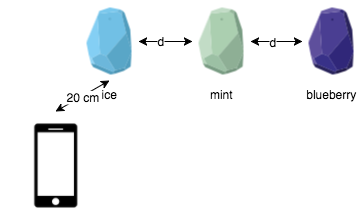
\includegraphics[width=0.5\textwidth, keepaspectratio]{images/nearest_beacon}
    \caption[Layout for experiments of nearest beacon]{Layout used for the experiments to get the accuracy of the distance value}
    \label{fig:layout_experiments_nearest_beacon}
\end{figure}

\subsection{Results}
\label{sub:evaluation_nearest_beacon_results}
The mobile app for end users scans for beacons but only requests data for the nearest one. To get the nearest one, it has to rely on the signal strength to calculate the distance. We performed 4 experiments in order to try to get the accuracy of the mechanism that calculates the distance that the mobile device is from a given beacon.
The results of these experiments are summarized in Table~\ref{tab:results_nearest_beacon} where it is possible to see for each beacon how many times it was detected as the nearest one.

Taking into account the layout that was used (see Figure~\ref{fig:layout_experiments_nearest_beacon}), the nearest beacon was the one with name ``ice'' (the blue one).
From Table~\ref{tab:results_nearest_beacon} it was possible to create the graphic shown in Figure~\ref{fig:results_experiments_nearest_beacon} which shows that, as we increase the distance between beacons, the accuracy to detect the nearest beacon also increases.
In all experiments, this beacon was detected as the nearest one at least 50\% off all scans performed.
The only difference between all experiments is the distance between beacons.
We can conclude that, it is recommended that the beacons are at least, 1.5m or 2m distant from each other.

\includeTable{results_nearest_beacon}

\begin{figure}[!ht]
  \centering
    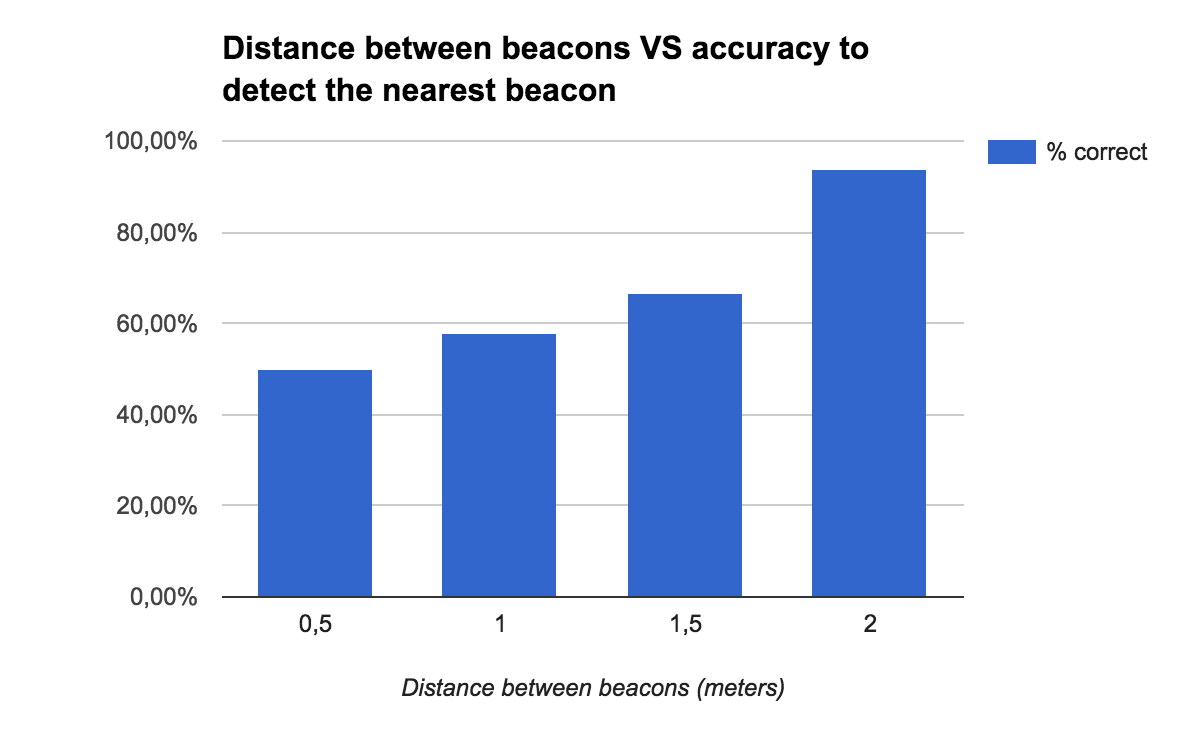
\includegraphics[width=0.5\textwidth, keepaspectratio]{images/results_nearest_beacon}
    \caption[Distance between beacons vs Accuracy]{Relation between distance between beacons and accuracy to detect the nearest beacon}
    \label{fig:results_experiments_nearest_beacon}
\end{figure}

In an environment where the beacons are close to each other, our solution might not work as expected.
For instance, in the previously described Smart Restaurant example
the tables should not be close to each other. This is not always possible because some restaurants try to optimize space and have tables as much close to each other as possible.
In the Smart Museum example two objects in a given exhibition should not be close to each other.
Otherwise, the visitor would be notified about an object and he might be looking at another one.
This error can be avoided using solutions such as Estimote Indoor \gls{SDK}\footnote{http://github.com/Estimote/iOS-Indoor-SDK} that can be used to obtain the physical location of the user inside a building or a room.
% How it works
However, using it requires the user to place beacons around the room.
Then, he needs to walk through the room in order for the app that is using the \gls{SDK} to get the needed data to do the mapping.
Only after this mapping it is possible to get the user's location.
It is only available for iOS.

\section{Energy Consumption}
\label{sec:evaluation_energy_consumption}
Another important aspect of this solution is the battery consumption.
Since our mobile app for end users runs on background to scan for nearby beacons, that can have a negative impact on the device's battery. If the user notices that the battery drains too fast, he will not use this solution.
We perfomed experiments to measure how much energy is drained only by our mobile app for end users.
Similar to section \ref{sec:evaluation_nearest_beacon} in the next sub sections we describe the metholodogy used and explain the results obtained in these experiments.

\subsection{Methodology}
\label{sub:evaluation_energy_consumption_methodology}
Table~\ref{tab:experiments_battery} outlines the experiments performed to evaluate the battery consumption.
Figure~\ref{fig:layout_experiments_battery_consumption} shows the layout used for this group of experiments.
We have used the same beacons as in the experiments described in section \ref{sec:evaluation_nearest_beacon}.
The beacons are equally distant, 25 cm, from each other.
The smartphone is at the same distance from the beacon in the middle, the green one named mint.
We performed six experiments.
In each one the app was turned on and ran for 1 hour in background mode scanning for beacons in order to discover nearby Smart Places.
The first two used \gls{WiFi} data connection.
The remaining used \gls{3G} mobile network.
Different data connection means can lead to different energy consumptions.
We need to understand which connection, \gls{WiFi} or \gls{3G}, drains more power.
If it is \gls{3G}, the user might only use our solution if he/she is connected to a \gls{WiFi} \gls{AP}.
We want our mobile app to be always turned on scanning for nearby Smart Places.
Using it only when \gls{WiFi} is available would make its usage very limited and the user would not take the full advantage of it because he/she needs be aware that a \gls{WiFi} \gls{AP} is available and turn the mobile app on again.
We tested two values for the interval between each scan, 5 minutes because it is the default value that the beacons library use in background mode, and 2 and half minutes.
The second value is half the first in order to see how much more power is drained when we set a smaller value for the interval between each scan.
Trying to find a smaller interval is important because it will reduce the probability that the user was not able to discover a nearby Smart Place.

The following scenarios were tested:
\begin{itemize}
  \item
  When the user stays in the same Smart Place the entire experiment;
  % Explain better
  \item
  When the user moves from one Smart Place to another, at each two and half minutes.
  % Explain better
\end{itemize}

\includeTable{experiments_battery}

\begin{figure}[!ht]
  \centering
    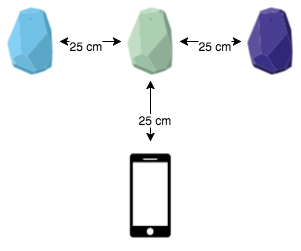
\includegraphics[width=0.5\textwidth, keepaspectratio]{images/experiments_battery_layout}
    \caption[Layout for experiments of battery consumption]{Layout used for the experiments to get the battery consumption}
    \label{fig:layout_experiments_battery_consumption}
\end{figure}

The mobile app for end users has a cache that stores the beacons that were already scanned.
This way, repeated communications with the backend are avoided.
Data communications, \gls{WiFi} or \gls{3G}, are the major source of battery drain as suggested in studies such as \cite{energy}.
To test both scenarios we would need more than three beacons spread along a big space.
Instead, we simulated the user walking passing by multiple Smart Places just by cleaning the cache, at each scan process.
This forced the app to make requests to the backend each time the three beacons were detected, allowing us to understand the impact of these requests on the power drain.
We used Battery Historian\footnote{https://developer.android.com/tools/performance/batterystats-battery-historian/index.html} to measure the power drain and how much data was transferred (sent and received). This tool allowed us to get the percentage of power drain.

\subsection{Results}
\label{sub:evaluation_energy_consumption_results}
% Tested first scenario
After we tested the first scenario, when the user stays in the same Smart Place we got the results shown in Table~\ref{tab:results_battery_stopped}, where we can see, for each variation of data connection type (\gls{WiFi} and \gls{3G}) and interval between each scan, the values obtained for power drain and data transferred.
From these results we obtained the graphic in Figure~\ref{fig:results_battery_stopped}.
% Concluded that the power drain is greater when using 3G
It is possible to see that using \gls{WiFi} we got no power drain.
However, using \gls{3G} it drained 0.29\% and 0,40\% of the total battery available.
After these first results we concluded that the biggest overhead comes from using \gls{3G} connection.

\includeTable{results_battery_stopped}

\begin{figure}[!ht]
  \centering
    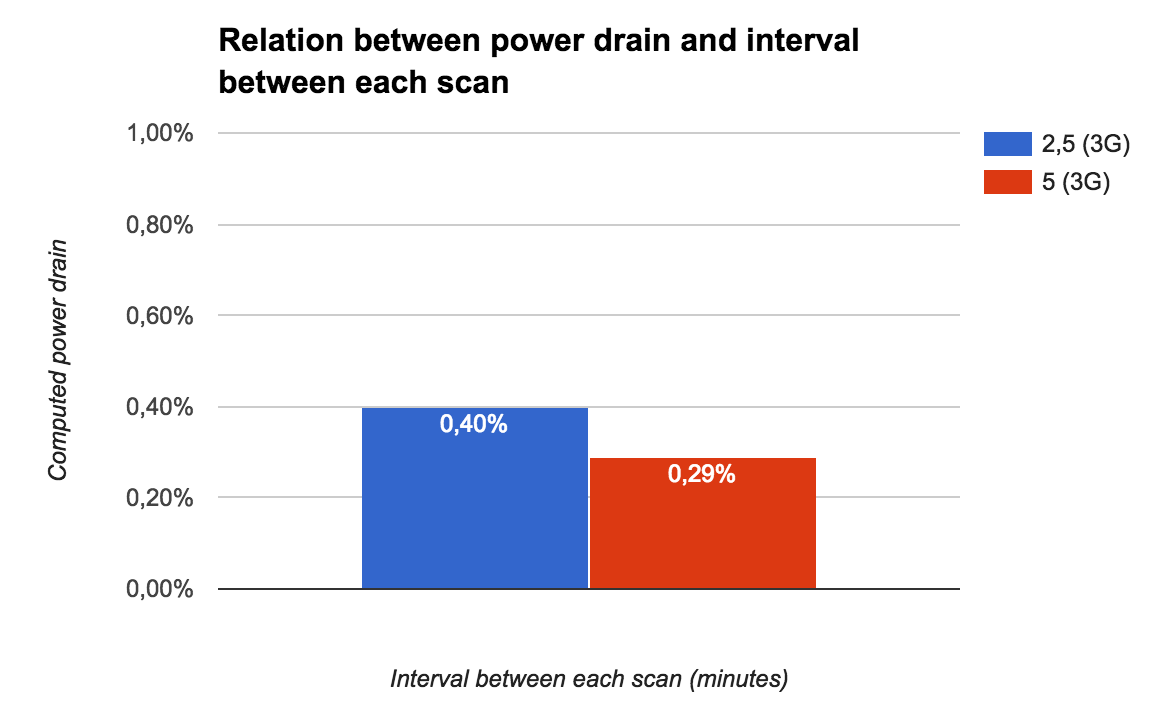
\includegraphics[width=0.8\textwidth, keepaspectratio]{images/results_battery_stopped}
    \caption[Power drain when the user does not move]{Relation between power drain and interval between each scan in the scenario where the user stays in the same Smart Place}
    \label{fig:results_battery_stopped}
\end{figure}

% Tested Facebook using 3G
After the first set of experiments we tested Facebook\footnote{http://play.google.com/store/apps/details?id=com.facebook.katana} since it is one of the popular apps and also has services running in background.
It is also known to be one of most power draining apps\footnote{http://www.forbes.com/sites/jaymcgregor/2014/11/06/facebook-and-instagram-are-killing-your-phones-battery-heres-a-simple-fix}.
We let it ran for 1 hour as we did in our first experiments.
While running Facebook, we used it to check our news feed in 5 minutes. The rest of the time the app was running in background.
Table~\ref{tab:results_facebook} summarizes the conditions and results of the test performed using Facebook app.
We used these values as a reference to compare with the power drain in the second scenario, that is, at each scan the user moves from one place to another which implies more requests to the backend.

\includeTable{results_facebook}

% Tested second scenario
Then, we performed the second set of experiments, that is, the second scenario where the user moves from one Smart Place to another.
Here, the app requests more data from the backend.
Table~\ref{tab:results_battery_walking}, shows the results for this scenario. Here, we got more power drain than in the previous scenario.
These results shows that, the more communication with the backend is required, more power our solution drains.
Once more, using \gls{WiFi}, we have got almost zero power drain.
However, similar to the results in the previous scenario, there is more power drain using \gls{3G}.
Graphic shown in Figure~\ref{fig:results_battery_walking} shows that, using two minutes and half of interval between each scan, we got more 0.71\% than using five minutes.
As happened before, there is more power drain when we decrease the interval between each scan.

% Compare with Facebook
In the worst case we obtained a power drain of 2.71\% which is approximately 71\% less than using Facebook in the same period of time.
Using this app as a reference in terms of apps that run services in background, we can say that the battery consumption is acceptable for a daily basis usage.

\includeTable{results_battery_walking}

\begin{figure}[!ht]
  \centering
    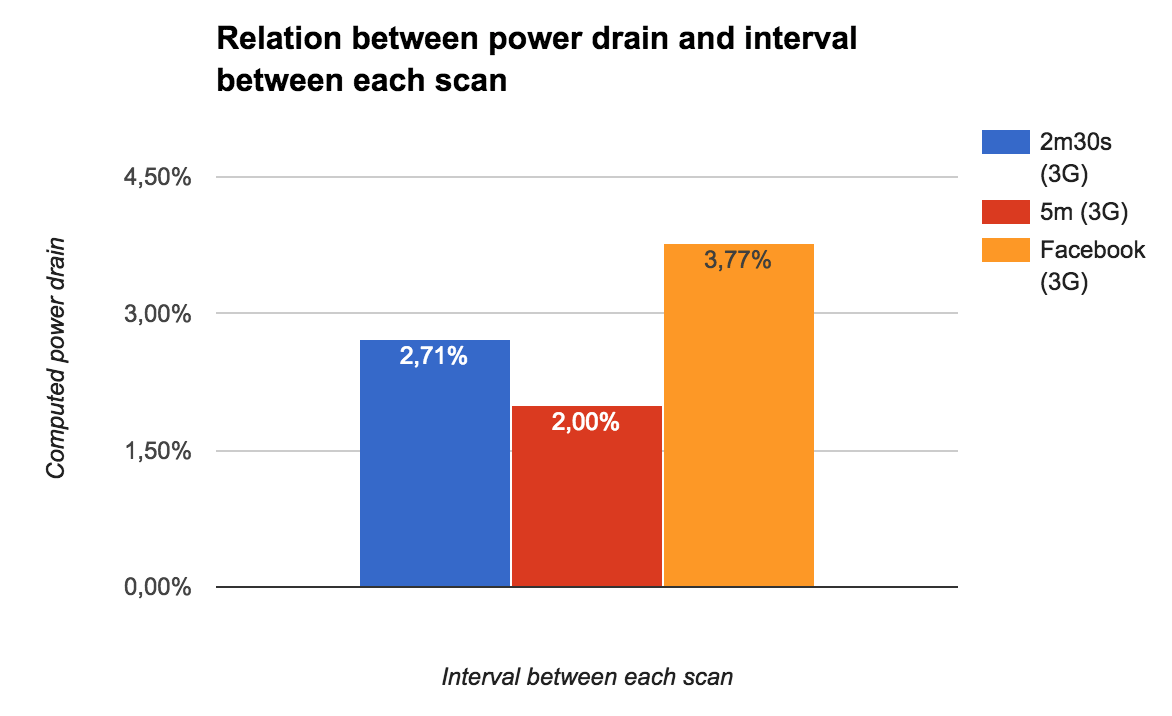
\includegraphics[width=0.8\textwidth, keepaspectratio]{images/results_battery_walking}
    \caption[Power drain when the user is moving]{Relation between power drain and interval between each scan in the scenario where the user moves along multiple Smart Places}
    \label{fig:results_battery_walking}
\end{figure}

% Dirty Hack to only start next section after showing the figures
\vfill

\section{Summary}
\label{sec:evaluation_summary}
% Setup
% -> Smartphone and 3 beacons of Estimote
% Two kinds of experiments
After developing the Smart Places solution, we performed an evaluation.
We have used a \tm{Motorola} Moto G smartphone and three beacons from \tm{Estimote} and we performed two sets of experiments.

% Nearest beacon
% -> What and why
% -> Comment results
The mobile app for end users scans for nearby beacons and requests information from the backend.
Our experiments showed that, to build applications that rely on detecting the nearest beacon, the beacons need to be, at least, 1.5m distant from each other.
As we raise the distance between beacons, the nearest beacon is successfully detected.

% Energy consumption
% -> What and why
% -> Comment results
The mobile app for end users scans for nearby beacons in background.
As any service running in background, it can introduce an overhead in terms of energy consumption.
We performed a set of experiments to get the power drain and data transferred (sent and received) by the mobile app.
We have tested two different scenarios. A scenario where the user stays in the same Smart Place and another one where he is always moving from one Smart Place to another.
Each experiment runned for one hour with a scanning period of 5 minutes or 2 and 30 seconds.
For each scenario, we tested \gls{WiFi} and \gls{3G} as data connection means.
The results showed that the power drain is bigger when using \gls{3G}. When using \gls{WiFi}, the power drain is almost zero.
In the scenario where the user does not move, the power drain is less than 1\%.
However, in the scenario where the user is always moving, which implies more requests to the backend, because new Smart Places are detected in each new scan, the power drain can be more than 2\%.
% Compare with Facebook and Facebook Messenger
We have measured the power drain of Facebook app, because it is one of the popular apps and also have services running in background.
The power drain of this app was used as a reference in order to compare with our solution in the worst case, when it needs to make requests to the backend in each scan.
Comparing the worst power drain in our solution with the Facebook app, we can say that the battery consumption of our solution is acceptable but needs to be improved.
